%
% teil1.tex -- Beispiel-File für das Paper
%
% (c) 2020 Prof Dr Andreas Müller, Hochschule Rapperswil
%
% !TEX root = ../../buch.tex
% !TEX encoding = UTF-8
%
\section{Gausssche Krümmung
\label{mongeampere:section:teil1}}
\kopfrechts{Gausssche Krümmung}
Damit wir verstehen, wie die monge-ampèresche Gleichung mit der 
Krümmung einer Fläche zusammenhängt, brauchen wir zuerst eine Methode diese 
Krümmug zu beschreiben.
Die Herleitungen in diesem Kapitel basieren auf \cite{mongeampere:smirnow}.
Wir betrachten dabei die Fläche
\begin{equation*}
  x = \varphi(u,v), \quad y = \psi(u,v), \quad z = \omega(u,v).
%  \label{mongeampere:areaparam}
\end{equation*}
Die Fläche kann man in der Parameterform auch als Radiusvektor
\index{Parameterform}%
\begin{equation*}
  \vec r (u, v) =
  \begin{pmatrix}
    x(u,v) \\
    y(u,v) \\
    z(u,v). \\
  \end{pmatrix}
%  \label{mongeampere:rad}
\end{equation*}
schreiben.
Leitet man diesen Radiusvektor nach den Parametern $u$ und $v$ ab, bekommnt man zwei Tangentialvektoren
$\vec r_u$ und $\vec r_v$,
mit welchen die Flächennormale 
\index{Flachennormale@Flächennormale}%
\begin{equation}
  \vec m = \frac{\vec r_u \times \vec r_v}{\!\sqrt{(\vec r_u \times \vec r_v)^2}} 
  \label{mongeampere:norm}
\end{equation}
beschrieben werden kann, wobei $(\cdot)^2$ für das Skalarprodukt eines Vektors mit sich selber steht.

\subsection{Erste Fundamentalform
\label{mongeampere:subsection:finibus}}
Die \emph{erste Fundamentalform} beschreibt die innere Geometrie einer Fläche.
\index{erste Fundamentalform}%
\index{Fundamentalform!erste}%
Betrachtet man das Quadrat des Bogendifferential einer auf der Fläche 
\index{Bogendifferential}%
beschriebenen Kurve $S(u,v)$ so ist 
\begin{equation*}
  \begin{split}
    d s^2 &= d x^2 + d y^2 + d z^2 \\
          &= \biggl(\frac{\partial x}{\partial u}\,d u + \frac{\partial x}{\partial v}\,d v  \biggr)^2
          + \biggl(\frac{\partial z}{\partial u}\,d u + \frac{\partial z}{\partial v}\,d v  \biggr)^2
          + \biggl(\frac{\partial z}{\partial u}\,d u + \frac{\partial z}{\partial v}\,d v  \biggr)^2.
  \end{split}
%  \label{mongeampere:bogdiff}
\end{equation*}
Rechnet man die Klammern aus, erhält man 
\begin{equation*}
    d s^2 = E(u,v) \,d u^2 + 2F(u,v) \,d u \,d v + G(u,v)\,d v^2
    %\label{mongeampere:1fundform}
\end{equation*}
mit
\begin{equation*}
\begin{aligned}
     E(u,v) &= \biggl(\frac{\partial x}{\partial u} \biggr)^2 +
     \biggl(\frac{\partial y}{\partial u} \biggr)^2 +
     \biggl(\frac{\partial z}{\partial u} \biggr)^2 
            &&= \vec r_u^2\\
     F(u,v) &= 
     \frac{\partial x}{\partial u} \cdot \frac{\partial x}{\partial v} +
     \frac{\partial y}{\partial u} \cdot \frac{\partial y}{\partial v} +
     \frac{\partial z}{\partial u} \cdot \frac{\partial z}{\partial v}
            &&= \vec r_u \cdot \vec r_v \\
      G(u,v) &= \biggl(\frac{\partial x}{\partial v} \biggr)^2 +
     \biggl(\frac{\partial y}{\partial v} \biggr)^2 +
     \biggl(\frac{\partial z}{\partial v} \biggr)^2 
             &&= \vec r_v ^2
  %\label{mongeampere:1fundbed}
\end{aligned}
\end{equation*}
Diese Formulierung des Bogendifferentials ist als erste Fundamentalform bekannt.
Man kann sie auch in Form des metrischen Tensors 
\begin{equation*}
  g_{ij} = \begin{pmatrix}
    E & F \\
    F & G \\
  \end{pmatrix}
  %\label{mongeampere:erstmettens}
\end{equation*}
beschreiben.

Die Koeffizienten der ersten Fundamentalform können auch für das Flächenelement mit
\begin{equation}
  d S = |\vec r_u \times \vec r_v|\,d u \,d v = \!\sqrt{EG-F^2} \,d u \,d v.
  \label{mongeampere:ds}
\end{equation}
verwendet werden.

\subsection{Zweite Fundamentalform}
Die \emph{zweite Fundamentalform} befasst sich mit der äusseren Geometrie einer 
\index{zweite Fundamentalform}%
\index{Fundamentalform!zweite}%
Fläche und beschreibt, wie sich die Tangente entlang einer Flächenkurve verändert.
Dafür betrachten wir wieder die Kurve $S(u,v)$ mit einem Tangentialeinheitsvektor 
$\vec t$.
Da die Kurve auf der Fläche liegt, ist $\vec t$ in jedem Punkt senkrecht auf der 
Flächennormale $\vec m$, womit $\vec t \cdot \vec m = 0$ gilt. 
Berechnen wir nun 
\begin{equation*}
  \frac{d }{d s}(\vec t \cdot \vec m),
  %\label{mongeampere:2fund0}
\end{equation*}
erhalten wir mit der Produktregel
\begin{equation}
  \frac{d \vec t}{d s} \cdot \vec m + \vec t \cdot \frac{d \vec m}{d s} = 0. 
  \label{mongeampere:2fund1}
\end{equation}
Der Term $d \vec t / d s = \varrho^{-1} \vec n$ beschreibt einen Vektor in Richtung der Kurvennormalen 
$\vec n$ mit der Länge $\varrho^{-1}$, welche den inversen Krümmungsradius der Kurve 
\index{Krummungsradius@Krümmungsradius}%
darstellt.
Somit können wir \eqref{mongeampere:2fund1} umformen nach
\begin{equation}
  \frac{\vec n \cdot \vec m}{\varrho} = - \frac{d \vec r \cdot d \vec m }{d s^2},
  \label{mongeampere:2fund2}
\end{equation}
Rechnet man den Zähler als Funktion der Parameter $u, v$ aus, erhält man die zweite 
Gausssche Fundamentalform
\begin{equation*}
  \mathrm{I\!I} = d \vec r \cdot d \vec m  = L(u, v) \,d u^2 + 2 M (u,v) \,d u \,d v + N(u,v) \,d v^2.
  %\label{mongeampere:2fund}
\end{equation*}
mit den Koeffizienten
\begin{align*}
  L &= \vec r_{uu} \cdot \vec m \\ 
  M &= \vec r_{uv} \cdot \vec m \\
  N &= \vec r_{vv} \cdot \vec m.
  %\label{mongeampere:2fundkoef}
\end{align*}
Die zweite Fundamentalform beschreibt, wie stark sich die Fläche an einem Punkt
von der Tangentialebene entfernt, wenn sich die Parameter etwas ändern.
\index{Tangentialebene}%
In \eqref{mongeampere:2fund2} haben wir die zweite Fundamentalform in Richtung einer Flächenkurve mit
dem Quadrat ihres Bogendifferentiales normalisiert.
Damit erhielten wir den Anteil der Krümmung der Flächenkurve, die von der Krümmung der Fläche kommt.

\subsection{Krümmung}
Um den Begriff der Krümmung auf einer Fläche etwas besser zu verstehen,
untersuchen wir die Krümmung von Normalenschnitten.
\index{Normalenschnitt}%
Ein \emph{Normalenschnitt} ist die Schnittkurve, zwischen der Fläche und der Ebene, welche durch einen Vektor auf 
\index{Schnittkurve}%
der Tangentialebene der Fläche und der Flächennormalen aufgespannt wird.
\begin{figure}
  \begin{center}
    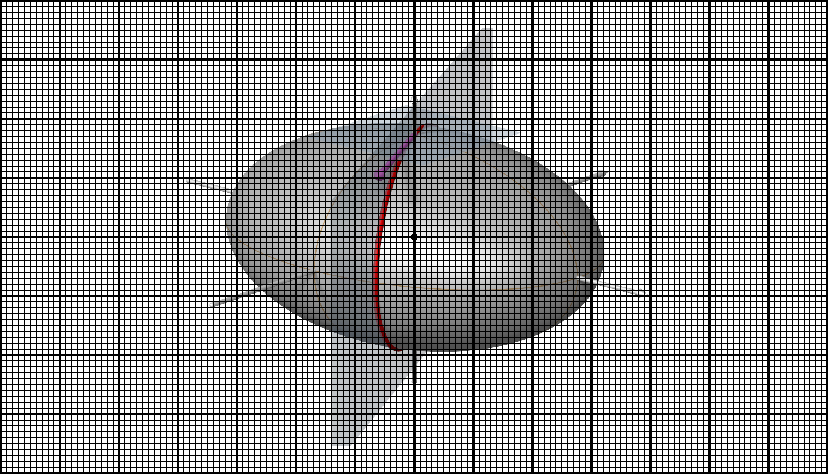
\includegraphics[width=0.95\textwidth]{papers/mongeampere/images/schnittkurven.pdf}
  \end{center}
  \caption{Schnittkurve auf einem Ellipsoid. Der Tangentialvektor $\vec t$ und die Flächennormale $\vec m$ spannen eine Ebene auf, 
  deren Schnitt mit der Fläche die Schnittkurve $y(t)$ ergibt. In Gelb sind die Parameterkurven von $u$ und $v$ dargestellt.}\label{mongeampere:fig:schnitt}
\end{figure}
In Abbildung \ref{mongeampere:fig:schnitt} ist ein Beispiel einer solchen Schnittkurve zu sehen.
Die Schnittkurve ist nur von der Richtung des Tangentialvektors abhängig, welche durch das Verhältnis von $d u$ und $d v$ charakterisiert wird.
Da die Normale eines Normalenschnittes bis auf das Vorzeichen gleich der Flächennormale ist, ist der 
Krümmungsradius
\begin{equation}
  \frac{1}{R} = \pm \frac{L \,d u^2 + 2 M \,d u\,d v + N \,d v^2}
                  {E \,d u^2 + 2F \,d u \, d v + G\,d v^2}.
  \label{mongeampere:normkrum}
\end{equation}
Diese Formulierung erlaubt uns, ein paar Eigenschaften der Fläche zu bestimmen.
Da der Nenner $d s^2$ entspricht, ist er immer positiv. 
Teilen wir den Zähler durch $d u^2$ erhalten wir den quadratischen Term
\begin{equation}
   L + 2M \frac{d v}{d u} + N \frac{d v^2}{d u ^2}.
  \label{mongemapere:dsik}
\end{equation}
Untersucht man die Diskriminante dieses Terms ergeben sich drei Fälle:
\index{Diskriminante}%
\begin{enumerate}
  \item $M^2 - LN < 0$: Das Vorzeichen des Krümmungsradius ändert sich nicht, somit geht die Krümmung für alle 
    Flächennormalen in dieselbe Richtung. 
    Ein solcher Punkt wird \emph{elliptisch} genannt. Ein Beispiel ist, wie der 
\index{elliptischer Punkt}%
\index{Punkt!elliptisch}%
\index{Ellipsoid}%
    Name schon vermuten lässt, ein Ellipsoid.
  \item $M^2 - LN > 0$: Das Vorzeichen des Krümmungsradius ändert sich, somit wechselt die Richtung der Krümmung.
    Ein solcher Punkt wird \emph{hyperbolisch} genannt. Ein Beispiel ist ein Sattelpunkt, wie auf einem einschaligen Hyperboloid.
\index{einschaliges Hyperboloid}%
\index{Hyperboloid}%
\index{hyperbolischer Punkt}%
\index{Punkt!hyperbolisch}%
  \item $M^2 - LN = 0$: Das Vorzeichen des Krümmungsradius ändert sich nicht, jedoch wird der Radius für einen 
    bestimmten Normalenschnitt null. 
    Ein solcher Punkt wird \emph{parabolisch} genannt. Eine parabolische Fläche ist die Mantelfäche eines Zylinders. 
\index{Mantelflache@Mantelfläche}%
\index{Zylinder}%
\index{parabolischer Punkt}%
\index{Punkt!parabolisch}%
\end{enumerate}
In Abbildung~\ref{mongeampere:arten} sind Beispiele zu den Flächentypen zu sehen.
\begin{figure}
	\centering
\begin{tikzpicture}[>=latex,thick]
	\pgfmathparse{12.6/6}
	\xdef\h{\pgfmathresult}
	\def\l{1.8}
	\begin{scope}[xshift=-4.2cm]
		\clip ({-\h},{-\l-0.7}) rectangle (\h,\l);
		\node at (-0.05,0) {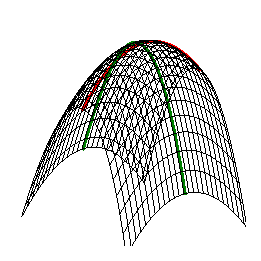
\includegraphics[width=4.8cm]{papers/mongeampere/fig/ellip.pdf}};
		%\draw[color=red] ({-\h},{-\l}) rectangle (\h,\l);
		\node at (0,-2.36) {(a)};
	\end{scope}
	\begin{scope}
		\clip ({-\h},{-\l-0.7}) rectangle (\h,\l);
		\node at (-0.15,0) {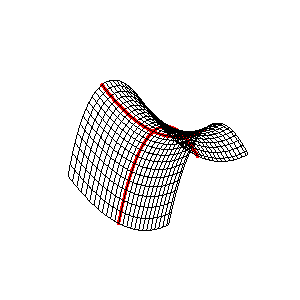
\includegraphics[width=4.8cm]{papers/mongeampere/fig/saddle.pdf}};
		%\draw[color=red] ({-\h},{-\l}) rectangle ({\h},\l);
		\node at (0,-2.36) {(b)};
	\end{scope}
	\begin{scope}[xshift=4.2cm]
		\clip ({-\h},{-\l-0.7}) rectangle (\h,\l);
		\node at (0.05,0) {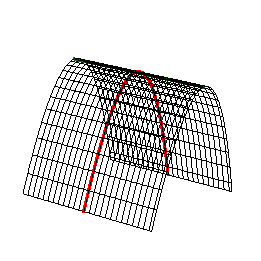
\includegraphics[width=5.0cm]{papers/mongeampere/fig/para.pdf}};
		%\draw[color=red] ({-\h},{-\l}) rectangle (\h,\l);
		\node at (0,-2.36) {(c)};
	\end{scope}
\end{tikzpicture}
%	\subfigure[]{
%		\label{mongeampere:ellip}
%		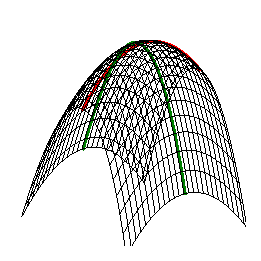
\includegraphics[width=0.32\textwidth]{papers/mongeampere/fig/ellip}}
%	\subfigure[]{
%		\label{mongeampere:sattel}
%		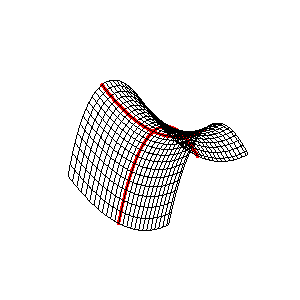
\includegraphics[width=0.32\textwidth]{papers/mongeampere/fig/saddle}} 
%	\subfigure[]{
%		\label{mongeampere:para}
%		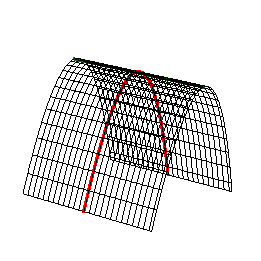
\includegraphics[width=0.32\textwidth]{papers/mongeampere/fig/para}}
	\caption{(a) Elliptischer Punkt (b) Hyperbolischer Punkt  (c) Parabolischer Punkt. In rot und grün sind die jeweiligen Hautpkrümmungen zu sehen.}
	\label{mongeampere:arten}\end{figure}
\subsubsection{Hauptkrümmungsradien}
Die Hauptkrümmungsradien an einem Punkt einer Fläche sind definiert als der kleinste und grösste Krümmungsradius an diesem Punkt.
Anhand des Ausdrucks \eqref{mongeampere:normkrum} lassen sich die beiden Hauptkrümmungsradien berechnen.
Dafür leiten wir den Term nach den Tangentenrichtungen $\frac{d v}{d u}$ und $\frac{d u}{d v}$ ab.
Mit etwas Umformen erhalten wir die quadratische Gleichung
\begin{equation*}
  (EG - F^2)\frac{1}{R^2} + (2FM - EN - GL)\frac{1}{R} + (LN-M^2) = 0.
  %\label{mongeampere:mainkrum}
\end{equation*}
Die Lösungen dieser Gleichung sind die beiden invertierten Hauptkrümmungsradien $R_1^{-1}$ und $R_2^{-1}$.
Wie wir aber im folgenden Abschnitt sehen werden, brauchen wir für die gausssche Krümmung die Gleichung nicht 
zu lösen.

\subsection{Gausssche Krümmung}
Die Krümmung wie wir sie in \eqref{mongeampere:2fund2} beschrieben haben hat das Problem, dass
ihr Vorzeichen abhängig von der Normalenrichtung ist.
Die \emph{gausssche Krümmung} ist ein Krümmungsmass, welches von solchen Faktoren unabhängig ist.
\index{gausssche Krummung@gausssche Krümmung}%
Sie is definiert als 
\begin{equation}
  K = \frac{1}{R_1 R_2} = \frac{LN-M^2}{EG-F^2}.
  \label{mongeampere:gausskrumm}
\end{equation}
Da sie die beiden Hauptkrümmungsradien multipliziert, ist sie immer positiv, wenn 
beide Krümmungradien das gleiche Vorzeichen haben, und negativ, falls sie sich unterscheiden.
Ausserdem lässt sich anhand des Vorzeichens bestimmen, ob ein Punkt elliptisch, hyperbolisch oder parabolisch 
ist, da die Diskriminante von \eqref{mongemapere:dsik} im Zähler ist.

Eine interessante Eigenschaft, welche Gauss als \emph{Theorema egregium} publiziert hat, ist, dass
\index{Theorema Egregium}%
die gausssche Krümmung mit den Koeffizienten der ersten Fundamentalform und ihren Ableitungen beschrieben werden kann.
Das bedeutet, dass die innere Geometrie einer Fläche bestimmt, welche gausssche Krümmung sie hat.
Im Umkehrschluss folgt, dass sich eine Fläche nicht auf eine andere Fläche mit einer anderen gaussschen Krümmung abbilden
lässt, ohne das Längen oder Winkel gestreckt werden.
Dieses Theorem erklärt also, wieso es keine längen- und winkeltreue flache Abbildungen der Erdoberfläche gibt.

